\documentclass[10pt]{report}
\usepackage{ifthen}
\usepackage{tikz}
% Optional PGF libraries
%\usetikzlibrary {arrows}
%\usetikzlibrary {snakes}
\usetikzlibrary{arrows}
\usetikzlibrary{decorations.pathmorphing}
\usetikzlibrary{backgrounds}
%\usetikzlibrary{placements}
\usetikzlibrary{fit}
\usepgflibrary{shapes.geometric}
\usetikzlibrary[shapes.misc]
\usetikzlibrary{positioning}
\usetikzlibrary{scopes}
\usepackage{amsopn}
\usepackage[fleqn,reqno]{amsmath}
%\usepackage[fleqn,tbtags]{amsmath}
\usepackage{mathtools}

\usepackage{hyperref}
\hypersetup{
%backref=false,
pdfdisplaydoctitle=true,
%pdfpagelayout=TwoColumnLeft,
pdffitwindow=true,
pdfpagetransition=Dissolve,
pdfpagemode=UseOutlines,
pdfnewwindow=true,
pdfstartpage=10,
colorlinks=true,
linkcolor=blue
}
\title{HmiGraphics}
\date{}

\makeatletter
\renewcommand{\@makechapterhead}[1]{%
\vspace*{50 pt}%
{\setlength{\parindent}{0pt} \raggedright \normalfont
\bfseries\Huge#1
\par\nobreak\vspace{40 pt}}}
\makeatother
\begin{document}

%\maketitle
%\begin{titlepage}
%\begin{center}
%\
%\vspace{10ex}
%
%{\Huge The HMIGraphics packages}
%\vspace{3ex}
%
%{\large Design and documentation for the HmiGraphics Java packages.}
%\end{center}
%\end{titlepage}

\setcounter{chapter}{0}

\ifx \hmigraphicsreportdir \undefinedmacro \def \hmigraphicsreportdir{.} \fi
\ifx \webserver \undefinedmacro \def \webserver{http://elckerlyc.sourceforge.net/javadoc/Hmi/} \fi
\chapter{The HmiGraphics packages}
The HmiGraphics and HmiAnimation packages constitute a framework for 3D graphics and animation, based upon Java and OpenGL.
This document describes the global structure of the various packages inside HmiGraphics and HmiAnimation.
The subdivision into HmiGraphics and HmiAnimation is largely based on the project structure used by build tools
like ant, Eclipse, and Netbeans. For an overview of the Hmi project structure, see \cite{hmiprojectstructure}

See the \href{\webserver}{javadoc}.



\section{Package overview}
The current contents of HmiGraphics and HmiAnimation is as follows:

\begin{itemize}
\item hmi.animation:
Deals with virtual objects, in particular animation of such objects. It defines a simple hierarchy of
virtual objects, by means of VJoints, primarily used for skeleton based animation of human avatars.
a virtual environment. Of course it is intended to be used in combination with the hmi.graphics packages,
but in principle it can be build and used independently.
\item hmi.graphics.collada:
Deals with reading (and to some extent writing) graphics files according to the Collada standard.
Apart from reading, it includes a sub package hmi.graphics.collada.scenegraph, for translating Collada descriptions into
hmi.graphics.scenegraph descriptions.
\item hmi.graphics.geometry:
Utility class, dealing with some purely geometric algorithms.
\item hmi.graphics.opengl:
Deals with actual rendering OpenGL based 3D graphics.
%It defines counterparts of some classes of the
%scenegraph package. For instance, we have the GLBasicMesh class which is sort of the hmi.graphics.opengl counterpart
%for the hmi.graphics.scenegraph GMesh class.
Although hmi.graphics.opengl is OpenGL based, it is still independent
of the  particular Java OpenGL binding or implementation. Currently there are two such OpenGL bindings: Jogl and LWJGL.
Each of these has its own package (hmi.graphics.jogl, hmi.graphics.lwjgl), and one of them must be used in combination with hmi.graphics.opengl.
hmi.graphics.opengl itself has a few sub packages:
\begin{itemize}
\item hmi.graphics.opengl.state: Contains classes for dealing with the OpenGL state management.
\item hmi.graphics.opengl.geometry: Defines a few utility classes for rendering simple geometry, like spheres, boxes, and lines.
\item hmi.graphics.opengl.scenegraph: Defines the translation from hmi.graphics.scengraph structures to hmi.graphics.opengl structures.
\end{itemize}

\item hmi.graphics.jogl and hmi.graphics.lwjgl are two packages that provide
actual OpenGL bindings, relying on native code in the form of windows dll files or Linux so files.
Both packages implement the GLRenderContext interface from hmi.graphics.opengl, and define
a simple Renderer.
Most of the JOGLContext and LWJGLContext code is generated, by means of a utility package hmi.graphics.gen.


\item hmi.graphics.scenegraph:
Defines scenegraph like structures for representing graphics data in a format independent of the external file format,
but also independent of the actual render technology being used.
\item hmi.graphics.util:
The usual package of our favorite ``utilities''.

\end{itemize}

Currently, there are a few more ``deprecated'' and/or temporary packages:
\begin{itemize}
\item hmi.graphics.colladatest:
Just for testing packages like collada, opengl, etcetera.
\item hmi.graphics.gen: used for generating files within  jogl and lwjgl implementations.
\item hmi.graphics.render
An attempt to create a platform neutral 3D renderer.
\end{itemize} 
%\section{Package dependencies}
We list the dependencies packages on our own hmi packages, as well as dependencies on non-standard
packages like Jogl or Ode.
Most packages depend on hmi.util and hmi.xml, and so we will not mention these for the sake of brevity.
\begin{itemize}
\item hmi.animation depends heavily on hmi.math. Otherwise it is quite independent, and it
 does explicitly \emph{not} depend on hmi.graphics packages,
nor on Jogl, LWJGL, or ODE.

\item hmi.graphics.scenegraph depends on hmi.math, hmi.graphics.geometry, and hmi.animation. It was designed to be independent of all other packages, in particular file format dependend packages like Collada, or render technology dependend packages like opengl, jogl, or lwjgl.

\item hmi.graphics.collada itself does not depend on other graphics packages. But it has a sub package hmi.graphics.collada.scenegraph that depends on hmi.graphics.scenegraph, hmi.graphics.collada, and hmi.math.

\item hmi.graphics.geometry does not depend on other packages

\item hmi.graphics.opengl depends on hmi.math, hmi.graphics.scenegraph, hmi.animation,
but \emph{not} on the Jogl or LWJGL.
The reference to hmi.animation is somewhat special:
the opengl package relies on VJoints for animation purposes. It is (only) here that the link between hmi.animation and
hmi.graphics is made.

\item hmi.graphics.jogl and hmi.graphics.lwjgl depend on hmi.graphics.opengl, as well as
on platform dependent dll files or so files, that reside inside the HmiGraphics/lib directory.
Inside the ant build files, the Jogl and LWJGL  dependencies can be denoted on
the ``dependencies'' line of \verb"build.properties", by means of the  \verb"Sun/jogl" or  \verb"LWJGL" tokens.
\item hmi.graphics.util, although small, combines various tools  and depends therefore on most other packages:
hmi.graphics.collada, hmi.graphics.opengl, and hmi.graphics.scenegraph.

\end{itemize}
%\section{The GLRenderContext: usage, implementation, and generation}
Rendering within the hmi.graphics package is OpenGL based. Several Java based implementations
and ``bindings'' for OpenGL exist. Currently, the most promising are Jogl (supported by Sun)
and LWJGL (very active community and some real commercial usage). Jogl is in a state of transition from a stable version based upon OpenGL 2.1 towards a new ``Jogl 2'' version that supports OpenGL 3.x. 
They all have much in common, since, basically, they are all just wrappers for the C functions from the OpenGL drivers.
At the same time, they differ enough so that one cannot serve as a ``drop in'' replacement for one of the others.
The answer to this unfortunate situation is (yet another) wrapper. (Fortunately, the wrapper is pretty straightforward and performance is not affected.)
Some of the differences between Jogl and LWJGL:
\begin{itemize}
\item Jogl represents the OpenGL context by means of an \emph{object} op type \verb"GL" that has a large number of methods, one for every relevant OpenGL function.  This is clearly the `object oriented'' style 
    and allows for more sophisticated handling of OpenGL by several processes concurrently. For instance, Jogl will
    (re-)acquire the OpenGL context  for every frame that is to be rendered. 
\item LWJGL on the other hand represents these OpenGL functions by means of \emph{static Java methods}, bundled in a few classes like \verb"GL11".
    The class names (\verb"GL11", \verb"GL12", ..., \verb"21") correspond to OpenGL versions $1.1, 1.2, ..., 2.1$.
    Each of them defines the methods for function introduced in that OpenGL version, which is nice if you want to keep track of the OpenGL version needed to run your application, but otherwise it's just an annoyance.  
\item In principle there would have been a one-to-one correspondence between the C functions for OpenGL and their Java counterparts, if Java would have dealt with pointers and arrays in the same style as within the C language. Such is not the case, and so each Java binding must somehow deal with function arguments like a pointer-to-float which is just the C representation of a float array parameter. There are some complications here, so there is no obvious solution, so, unavoidably,  Jogl and LWJGL have selected \emph{different} solutions.
    \begin{itemize}
     \item An ``array of floats'' is in C just a pointer to a float. That pointer points to the first element
     of the array, but by adding some ``offset'', it can point just as easily to some other starting point.
     \item An ``array of floats'' in Java can be represented as a Java float array, i.e. of type \verb"float[]".
     It can also be represented by means of a ``direct'' or ``indirect'' \verb"FloatBuffer" object. 
     \item Both Java float arrays and indirect \verb"FloatBuffers" are represented within the Java ``heap'', but direct \verb"FloatBuffers" are kept ``outside'' that heap. As a consequence, the Java native interface calls         can deal more efficiently with direct \verb"FloatBuffers" than with indirect buffers or float arrays. The flip side is that direct buffers are not automatically garbage collected, and although cpying large chunks of information from or to a direct buffer is ok, accessing individual buffer elements is not very efficient. (Basically, Java performs some checks when it passes information across the boundary of the Java virtual machine, for safety and security reasons). 
     \item Java float arrays have no means to represent ``offsets'' into an array the same way you can do this in C. But \verb"FloatBuffers" can represent such offsets by means of the current buffer position.
     \item Both Jogl and LWJGL use \verb"FloatBuffers" as the preferred way of representing C style float pointers. But Jogl also allows plain Java float arrays, as a convenience, whereas LWJGL suggest that you introduce a \verb"FloatBuffer" wrapper in such cases. When you do use an array in Jogl, you must also specify
         an ``offset'' in the form of a (long) integer, and as an ``extra'' argument for the Java method. 
    \end{itemize}
    
    
\end{itemize}
The \verb"GLRenderContext" interface from the hmi.graphics.opengl package (or more precisely, the \verb"GLBinding" sub-interface) has been introduced to get rid of the interface differences between Jogl and LWJGL. (It seems that the Jogl 2 interfaces introduce yet another variation, so we will capture that one as well).
The \verb"GLBinding" interface introduces a selection of the more useful OpenGL calls, and uses the more useful
 parameter conventions. So:
 \begin{itemize}
 \item Like Jogl, and unlike LWJGL, the \verb"GLBinding" interface represents the OpenGL conext by means of an Java object. The \verb"GLRenderContext" extends \verb"GLBinding", and adds a few render attributes, like the render ``pass''.
 \item There is one context, no annoying distictions between OpenGL versions.
 \item \verb"FloatBuffers" are preferred, but for a few cases float arrays are allowed as convenience method, but without the superfluous integer offset from Jogl. (When you really  want offsets, you want to use \verb"FloatBuffers" anyway)
 \end{itemize}
 
 \subsection{Generating the Java bindings}
 From the section above it should be clear that we have a number of Java classes and interfaces that need to be ``in sync'' so to say. These are:
 \begin{enumerate}
 \item \verb"GLRenderContext" and \verb"GLBinding.java" from hmi.graphics.opengl
 \item \verb"JOGLContext" from hmi.graphics.jogl
 \item \verb"LWJGLContext" from hmi.graphics.lwjgl
 \end{enumerate} 
 Rather than manually updating each of these files, they are being \emph{generated} from a common definitions file called \verb"GLF.def", located in hmi.graphics.opengl, plus a few short binding-specific header files. The \verb"GLF.def" files contains templates from which the three files above can be generated. The \verb"GLBinding.header", \verb"JOGLContext.header", and \verb"LWJGLContext.header" deal with the few things that could not be dealt with in a generic way.
 
 To be concrete:
 \begin{enumerate}
 \item \verb"GLBinding.java" is generated by running \verb"GenGLBinding" from the hmi.graphics.gen package.
 (\verb"GLRenderContext" simply extends \verb"GLBinding", so it us updated implicitly)
 \item \verb"JOGLContext" is generated by running \verb"GenJOGLContext" from hmi.graphics.gen
 \item \verb"LWJGLLContext" is generated by running \verb"GenLWJGLContext" from hmi.graphics.gen
 \end{enumerate}
 
 
  The format for the \verb"GLF.def" file is as follows:
  \begin{itemize}
  \item A line like :\\
  \verb"GL11  public void glClear(int mask);"\\
  denotes a simple OpenGL function \verb"glClear" with one int-typed argument called \verb"mask". 
  It is prefixed by \verb"GL11" to denote that it is an OpenGL 1.1 function. ( Jogl  will ignore this,
  but  LWJGL  needs it.)
  \item The two lines:\\
  \verb"GL11  public void glGetFloatv(int pname, FloatBuffer params);"
  \verb"GL11  public void glGetFloatv(int pname, float[] params);"\\
  denote two variations of the OpenGL function \verb"glGetFloatv", one with a \verb"FloatBuffer",
  one with a Java float array. Note that we have no Jogl-style array offset.
  For Jogl, the translation in JOGLContext.java becomes:\\
  \verb"public final void glGetFloatv(int pname, FloatBuffer params) "\\
  \verb"  { gl.glGetFloatv(pname, params); }"\\
  \verb"public final void glGetFloatv(int pname, float[] params) "\\
  \verb"  { gl.glGetFloatv(pname, params, 0); }"\\
  Whereas for LWJGL, we have inside LWJGLContext.java:\\
  \verb"public final void glGetFloatv(int pname, FloatBuffer params)  "\\
  \verb"  { GL11.glGetFloat(pname, params); }"\\
  \verb"public final void glGetFloatv(int pname, float[] params)  "\\
  \verb"  { GL11.glGetFloat(pname, FloatBuffer.wrap(params));}"\\
  
  \item Finally, we sometimes need some "hack" in cases like this line in \verb"GLF.def":\\
  \verb"GL11  public void glDrawElements"\\
  \verb"    (int mode, int bufcount, int buftype, IntBuffer indices);"\\
  For Jogl, this translated in straightforward manner:\\
  \verb"public final void glDrawElements"\\
  \verb"    (int mode, int bufcount, int buftype, IntBuffer indices)"\\
   \verb"   { gl.glDrawElements(mode, bufcount, buftype, indices); }"\\
   But for LWJGL, the fact that we use an \verb"IntBuffer" argument is used to infer the buftype and bufcount
   arguments. So the translation becomes:\\
   \verb" public final void glDrawElements"\\
   \verb"   (int mode, int bufcount, int buftype, IntBuffer indices) "\\
   \verb"   { GL11.glDrawElements(mode, indices); }"\\
  \end{itemize}
  
  This works only because of a "hack": the two parameter names \verb"bufcount" and \verb"buftype"
  are recognized as such when used in a parameterlist where also some buffer is used,
  and the LWJGL translation will omit them for the LWJGL translation. 
\section{Skeleton Structures for avatars}
An avatar that is to be used for (bodily) animation must
posses a \emph{skeleton} or \emph{bones} structure.
By this we do not mean a physical model or a visualization of
a real skeleton, but rather a structure consisting \emph{joints} and
\emph{segments} or \emph{bones} that is to be used for the purpose of animation.
See the picture in \autoref{figure:skeleton} for an example skeleton.
%\vspace{ex}
A skeleton consists of \emph{joints}, like the Pelvis or Spine nodes in the picture,
connected by means of \emph{segments} (or ``\emph{bones}''), shown here by means
of arrows connecting the joints. It will be clear that a skeleton is a rooted tree.
(For the example skeleton, the root node is the Pelvis node)




\begin{figure}

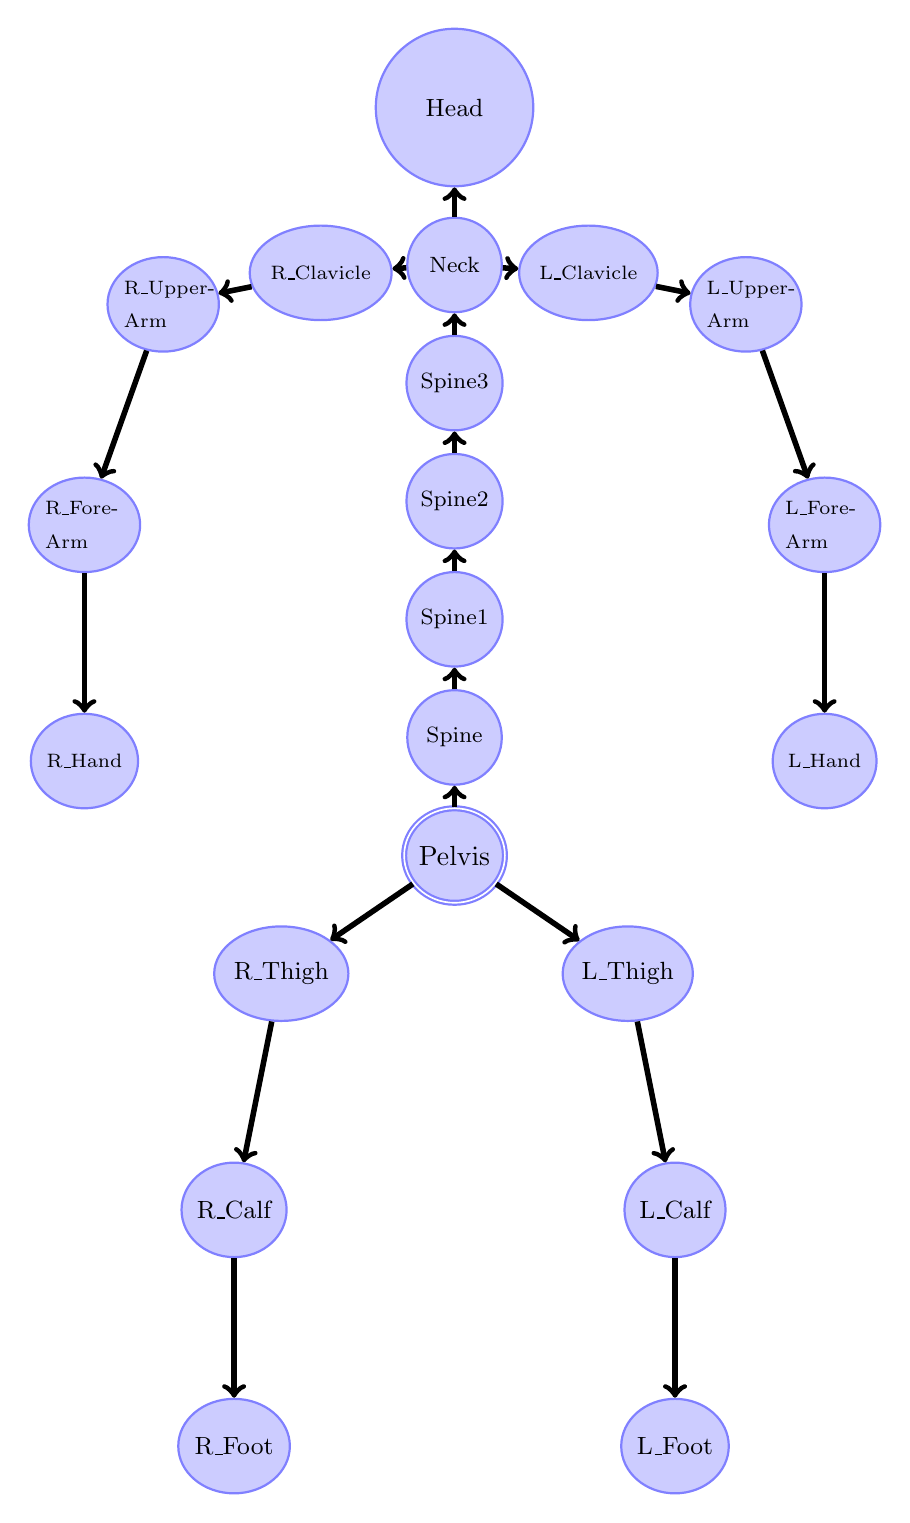
\begin{tikzpicture}
  [joint/.style={shape=ellipse,draw=blue!50,fill=blue!20, thick,
         inner sep=0pt, minimum width=12mm, minimum height=12mm}
  ]

 \path
   (0, 0) node (pelvis)            [joint, double] {Pelvis}
   {[current point is local] % start upper body branch, from pelvis
      ++(0, 1.5)   node (spine)      [joint]         {\footnotesize Spine}
      ++(0, 1.5)   node (spine1)     [joint]         {\footnotesize Spine1}
      ++(0, 1.5)   node (spine2)     [joint]         {\footnotesize Spine2}
      ++(0, 1.5)   node (spine3)     [joint]         {\footnotesize Spine3}
      ++(0, 1.5)   node (neck)       [joint]         {\footnotesize Neck}
      {[current point is local] % start head branch, from neck
         ++(0, 2.0) node (head)       [joint, minimum size=20mm] {\small Head}
      }
      {[current point is local] % start left arm branch, from neck
         ++(1.7, -0.1)   node (lclavicle)  [joint] {\scriptsize L\_Clavicle}
         ++(2.0, -0.4)   node (lupperarm)  [joint, text width=10mm] {\scriptsize L\_Upper\-Arm}
         ++(1.0, -2.8)   node (lforearm)   [joint,  text width=10mm] {\scriptsize L\_Fore\-Arm}
         ++(0.0, -3.0)   node (lhand)      [joint] {\scriptsize L\_Hand}
      }
      {[current point is local] % start right arm branch, from neck
         ++(-1.7, -0.1)  node (rclavicle)  [joint] {\scriptsize R\_Clavicle}
         ++(-2.0, -0.4)  node (rupperarm)  [joint, text width=10mm] {\scriptsize R\_Upper\-Arm}
         ++(-1.0, -2.8)  node (rforearm)   [joint,  text width=10mm] {\scriptsize R\_Fore\-Arm}
         ++(0.0,  -3.0)    node (rhand)    [joint] {\scriptsize R\_Hand}
      }
   }
      {[current point is local] % start left leg branch, from pelvis
         ++(2.2, -1.5) node (lthigh)  [joint] {\small L\_Thigh}
         ++(0.6, -3) node (lcalf)   [joint] {\small L\_Calf}
         ++(0, -3)   node (lfoot)   [joint] {\small L\_Foot}
      }
      {[current point is local] % start right leg branch, from pelvis
         ++(-2.2, -1.5) node (rthigh)  [joint] {\small R\_Thigh}
         ++(-0.6, -3) node (rcalf)   [joint] {\small R\_Calf}
         ++(0, -3)    node (rfoot)   [joint] {\small R\_Foot}
      }
   ;
   \begin{scope}[line width=2pt]
   \draw [->] (pelvis) -- (spine);
   \draw [->] (spine) -- (spine1);
   \draw [->] (spine1) -- (spine2);
   \draw [->] (spine2) -- (spine3);
   \draw [->] (spine3) -- (neck);
   \draw [->] (neck) -- (head);
   \draw [->] (neck) -- (lclavicle);
   \draw [->] (lclavicle) -- (lupperarm);
   \draw [->] (lupperarm) -- (lforearm);
   \draw [->] (lforearm) -- (lhand);
   \draw [->] (neck) -- (rclavicle);
   \draw [->] (rclavicle) -- (rupperarm);
   \draw [->] (rupperarm) -- (rforearm);
   \draw [->] (rforearm) -- (rhand);
   \draw [->] (pelvis) -- (lthigh);
   \draw [->] (lthigh) -- (lcalf);
   \draw [->] (lcalf) -- (lfoot);
   \draw [->] (pelvis) -- (rthigh);
   \draw [->] (rthigh) -- (rcalf);
   \draw [->] (rcalf) -- (rfoot);
   \end{scope}

\end{tikzpicture}
\caption{Example of a skeleton structure}\label{figure:skeleton}
\end{figure} 

\def\Alocal{\mathstrut^L\!A}


%\[
%{}^{14}_{2}\mathbf{C}^{5+}_{2} \quad
%\prescript{14}{2}{\mathbf{C}}^{5+}_{2} \quad
%\prescript{4}{12}{\mathbf{C}}^{5+}_{2} \quad
%\prescript{14}{}{\mathbf{C}}^{5+}_{2} \quad
%\prescript{}{2}{\mathbf{C}}^{5+}_{2}
%\]


\subsection{Affine and linear transforms}
Within this chapter by \emph{linear} transform we mean an ordinary linear mapping for 3D space, represented
by a $3\times 3$ matrix $M$.
A \emph{translation} $T$ is defined by a 3D translation vector $t$.
When we want to make this vector it explicit, we write $T_t$ for a translation operation.
As is well known, a translation operation $T$ is not linear, so cannot be represented by a $3\times 3$ matrix.
We often need the combination $A$ of a linear transform $M$ followed by a translation $T$, so $A=T\circ M = T\,M$.
Such a combination is called an \emph{affine} transform.
The combination in the reverse order, i.e. $M\,T = M\, T_t$ is also affine, since it is equivalent
to the affine transform $A = T_{t'} \, M$, where $t'=M(t)$.
As a consequence, a composition of affine transforms $A_0$ and $A_1$ is itself also affine:
%
\begin{gather}\label{affinecomposition}
A_0A_1 = T_{t_0}\,M_0\, T_{t_1}\, M_1 = T_{t_0}\,T_{M_0(t_1)}\,  M_0 \,M_1 =
T_{t'}M',\\
\text{where } t' = t_0 + M_0(t_1) \text{ and } M' = M_0\, M_1.\notag
\end{gather}
%

\noindent
A (non-degenerate) linear transformation can be an \emph{orthogonal} matrix $Q$
which for 3D spaces is either a pure \emph{rotation} $R$, or else a rotation combined with a \emph{reflection}.
(In the latter case it can represented, for instance, as $Q=R\,N$, where $R$ is a pure rotation,
and where $N$ is a reflection. For instance, one may choose $N$ to be $-I$.
Another important class of linear transforms is that of \emph{scaling}.
In the simplest case, a scaling matrix $S$ is just the ($3\times 3$) identity matrix multiplied
with a \emph{uniform scaling} factor $s$. A more complex case is when $S$ is a diagonal matrix
with three different scaling factors $s_x$, $s_y$, and $s_z$ on the diagonal, which represents axis-aligned
\emph{non-uniform scaling}. In the most complicated case, a scaling matrix $S$ is
not even diagonal, but it would be diagonal in some rotated coordinate system.
So it represents \emph{non-unform scaling along rotated axes}, a situation sometimes called \emph{skewing}.
An important result here is that by means of so  called \emph{polar decomposition}
any (non-degenerate) 3D matrix $M$ can be decomposed as $M=Q\, S$,
where $Q$ is orthogonal, and where $S$ is a scaling matrix. A nice property of polar decomposition
is that $Q$ is not just \emph{any} orthogonal matrix, but that among all orthogonal matrices it is the one
that is \emph{closest} to $M$. We conclude that, for our purpose, we may assume that
any linear 3D matrix $M$ has the form $R\,S$ where $R$ is a pure rotation and where $S$ is a scaling matrix,
possibly combined with a reflection operation.
Our affine transforms $A$ are therefore of the form $T\,R\,S$. Although $A$ is not a 3D linear transform
it \emph{can} be represented by a $4\times 4$ \emph{homogeneous} transform matrix.
So $A$ has a matrix with the $3\times 3$ matrix for $R\,S$ in the upper left part, the translation vector
$t$ for the translation $T$ in the rightmost column, and a
 bottom row of the form $(0,\;0,\;0,\; 1)$.



\subsection{Skeleton transforms}
\label{sect:skeletontransforms}

The main use of skeletons is that they organize a collection of transforms, one transform for every skeleton joint $J_i$.
Note: skeleton joints are sometimes called ``bones''. This terminology is slightly confusing since for others ``bones'' refer to
the skeleton segments in between the joints.


For joint transformations we must distinguish between a \emph{local transforms} $D_i$ versus the \emph{global transforms} $A_i$
associated with each joint $J_i$.
The local transform represents the transform caused by that single joint alone.
The global transform $A_i$, is the combined effect of all joints
on the path from the skeleton root up to and including the joint itself.
For instance, for the joint called L\_Forearm in the example skeleton,
the global matrix $A_\text{L\_Forearm}$ represent the rotations and translations
from the Pelvis joint, the various Spine joints, the Neck joint, the
L\_Clavicle joint, L\_UpperArm joint, and finally the L\_ForeArm joint itself.

The \emph{local transform} $D_i$  for a joint represents just the rotation $R_i$ (and possibly scaling $S_i$)
introduced by that joint alone, together with the translation that represents the vector $t$ from the parent
of that joint to the joint itself.
For instance, for the L\_ForeArm joint the local translation is represented by the vector from L\_UpperArm to L\_ForeArm.
Note that each $D_i$ is an affine transform.


 The idea of a skeleton is that joint transformations are build up hierarchically, following the tree
 structure of the skeleton. So, when some joint $J_i$ has joint $J_p$ as its parent,
 then $A_i = A_p \, D_i$, where $A_p$ is the transform associated with $J_p$,
 and where $D_i$ is the \emph{local} transform associated with joint $J_i$.
 For the special case of the root joint $J_0$, there is no parent, and we assume that in this case the
 transform $A_0$ is simply equal to the local transform $D_0$.
 For long chains of joint, we can thus factorize the transform $A$ of the end of the chain into
 the local transforms of the joints on the chain. For instance, for the example skeleton
 we can calculate the affine matrix of, say, the neck joint as follows:
 %
  \begin{equation}
  A_\textit{Neck} = D_\textit{Pelvis} \: D_\textit{Spine} \: D_\textit{Spine1} \: D_\textit{Spine2} \: D_\textit{Spine3} \:D_\textit{Neck}
  \end{equation}
%

\begin{figure}

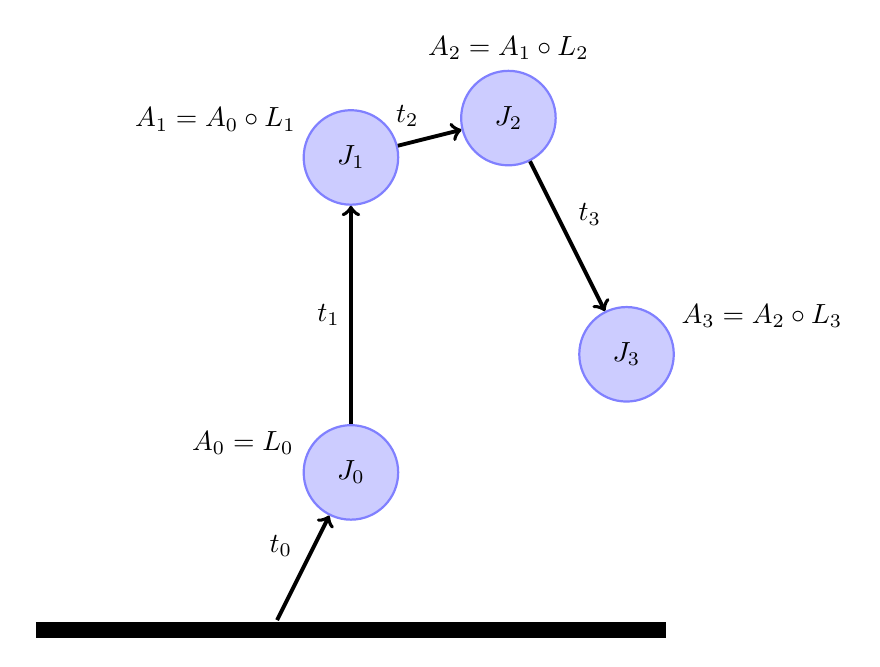
\begin{tikzpicture}
  [joint/.style={shape=ellipse,draw=blue!50,fill=blue!20, thick,
         inner sep=0pt, minimum width=12mm, minimum height=12mm},
  auto
  ]
   \begin{scope}[line width=6pt]

  \draw (-4,0) -- (4,0);
   \end{scope}
  \node (origin) [minimum size = 0] at(-1, 0) {  };
 \path
   (0, 2) node (j0)        [joint, label=170:{$A_0=L_0$}] {$J_0$}
  ++(0, 4)   node (j1)   [joint, label=160:{$A_1=A_0\circ L_1$}]         {$J_1$}
  ++(2, 0.5)   node (j2)    [joint, label=90:{$A_2=A_1\circ L_2$}]         {$J_2$}
  ++(1.5, -3)   node (j3)     [joint, label=20:{$A_3=A_2\circ L_3$}]         {$J_3$}

   ;
   \begin{scope}[line width=1.4pt]
   \draw [->] (origin) to node{$t_0$} (j0);
   \draw [->] (j0) to node{$t_1$}(j1);
   \draw [->] (j1) to node{$t_2$}(j2);
   \draw [->] (j2) to node{$t_3$}(j3);
   \end{scope}

\end{tikzpicture}
\caption{Part of a skeleton, with Translations $t_i$, Local Transforms $D_i$, and global transforms $A_i$}\label{figure:skeletonfragment}
\end{figure} 
For the smaller scale example from \autoref{figure:skeletonfragment}, we have:
%
\begin{equation}\label{eq:a3}
 A_3 = A_2\: D_3 = A_1 \: D_2\: D_3 = A_0\: D_1\:D_2\:D_3 = D_0\: D_1\:D_2\:D_3.
 \end{equation}
%
% WinEDT bug triggered by this line??:
%
\begin{figure}

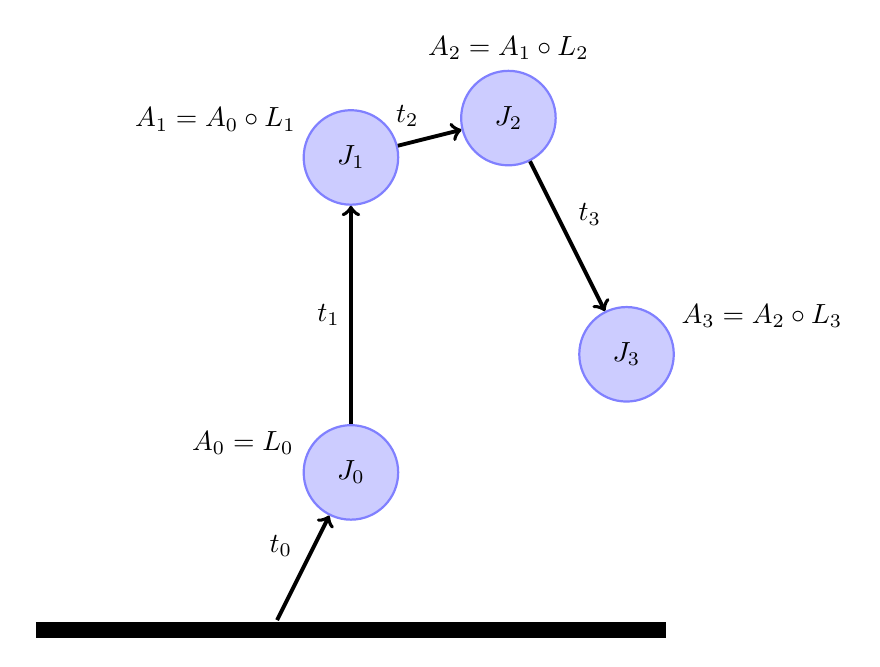
\begin{tikzpicture}
  [joint/.style={shape=ellipse,draw=blue!50,fill=blue!20, thick,
         inner sep=0pt, minimum width=12mm, minimum height=12mm},
  auto
  ]
   \begin{scope}[line width=6pt]

  \draw (-4,0) -- (4,0);
   \end{scope}
  \node (origin) [minimum size = 0] at(-1, 0) {  };
 \path
   (0, 2) node (j0)        [joint, label=170:{$A_0=L_0$}] {$J_0$}
  ++(0, 4)   node (j1)   [joint, label=160:{$A_1=A_0\circ L_1$}]         {$J_1$}
  ++(2, 0.5)   node (j2)    [joint, label=90:{$A_2=A_1\circ L_2$}]         {$J_2$}
  ++(1.5, -3)   node (j3)     [joint, label=20:{$A_3=A_2\circ L_3$}]         {$J_3$}

   ;
   \begin{scope}[line width=1.4pt]
   \draw [->] (origin) to node{$t_0$} (j0);
   \draw [->] (j0) to node{$t_1$}(j1);
   \draw [->] (j1) to node{$t_2$}(j2);
   \draw [->] (j2) to node{$t_3$}(j3);
   \end{scope}

\end{tikzpicture}
\caption{Part of a skeleton, with Translations $t_i$, Local Transforms $D_i$, and global transforms $A_i$}\label{figure:skeletonfragment}
\end{figure} 


%
We can decompose each local affine transform $D_i$ into a linear transform $L_i$ followed by
a translation $T_{t_i}$, thus: $D_i = T_{t_i}\: L_i$.
Using \eqref{affinecomposition} we can rearrange equation \eqref{eq:a3}.
%
\begin{gather}
A_3 = T_t \: L\\
 \text{where } t = t_0 + L_0(t_1) + L_0\,L_1(t_2) + L_0\,L_1\,L_2(t_3)\notag\\
 \text{and where } L= L_0\,L_1\,L_2\,L_3.\notag
\end{gather}
%
So the net effect of a ``chain'' of local affine transforms, from skeleton root up to some skeleton joint,
is equivalent to a single affine transform for that joint, which we have introduced before: it is the
\emph{global} transform for a joint.

\subsection{Weight blending}\label{sect:weightblending}



Skeletons can be controlled and used by animation software; in those cases, we are only concerned
with the local and global joint transforms. But skeletons are also used as an interface between
animation engines and graphics rendering engines.
In this case, the skeleton transforms are used
to transform geometry that is used for rendering objects, in particular for rendering human avatars.
The general idea is that there are one or more \emph{meshes}, each consisting of many polygons,
that model the  geometric shape of body parts.
There are two fundamentally different ways of doing this.
One rather simple approach is to cut an animated object into parts, each of which is then animated independently,
under the control of a single joint, dedicated to that part. For example, the ``blue guy'' avatar
uses this approach, and uses separate meshes for limbs and other body part.
The geometry associated with the elbow region of the body  is transformed exclusively
by the global affine transform for the elbow joint.
One of the advantages of this simple approach is that all mesh vertices inside a single body part
are transformed by the same affine matrix; a situation that suits the classical render pipeline
of graphics hardware, as well as the OpenGL and DirectX interfaces for that hardware.
 Simple or not, an unavoidable problem with this approach is that an avatar body as a whole
 shows seams at places where different body parts connect.

 An improved form of animating objects like human avatars is to use only \emph{one seamless mesh},
 and to use the skeleton transforms to deform by the following process:
 Each mesh vertex $v$ is transformed under the influence of one or more joints $J_{i_0}, \ldots, J_{i_n}$,
 with \emph{weights} $w_{i_0}, \ldots, w_{i_n}$ determining the relative influence of each joint.
 The exact set of joints and weights is unique for every individual vertex. Of course, one expects
 that most vertices will be controlled by a fairly low number of joints, typically one or two, and almost always less than four,
 all located in the neighborhood of the vertex. We would like to write down the transformation for some vertex $v$.
 We denote the global transform for joint $J_i$ by $A_i$ and, for simplicity, we assume that we have some vertex $v$
 that is influenced by joints $J_0, \ldots J_n$.
 The combined transform for $v$ using weight blending is defined as follows
%
\begin{equation}\label{eq:weightblending-simple}
 v' = \sum_{i=0}^{n} w_i\, A_i(v)
\end{equation}

\subsection{Bind poses}
Weight blending is an adequate animation method, but it requires both a suitable mesh as well
as a skeleton that ``fits'' into the mesh. A problem here is that designers of meshes and designers
of skeleton-based animations have slightly conflicting interests:
An animation system would prefer a skeleton that is in some well defined neutral pose
when all joint rotations are set to identity transforms. In that case all affine transforms
reduce to mere translations. The HAnim standard for skeleton based animation, for instance,
requires that in this situation the human avatar has a well defined pose where the body is upright,
arms are pointing downwards, fingers are pointing downwards, the thumbs have a $45^\circ$ degree orientation
relative to the fingers, etcetera.
The advantage of such a neutral pose is that an animation engine can put the avatar in some pose by setting well defined
rotations within joints.

Designers of nice looking avatar meshes though, prefer a \emph{different} pose, usually with the arms
horizontally stretched, also known as the ``T-pose''. The main reason here is that graphics designers
need to work on detailed graphic detail, and some areas like arm pits are difficult to reach and problematic when
the avatar is in the HAnim neutral pose, rather than the T-pose.
There are some variations of this ``T-pose'', for instance with the arms in a straight line but in a slightly lowered
position.

The result is that meshes and skeleton structures usually do \emph{not} automatically ``match'', and we need some
process called ``binding'' the mesh to the skeleton. One of the steps in the binding process is
that the skeleton, starting initially in its neutral pose, is put into ``bind pose'', by applying suitable
rotations for its joints. For example, for our HAnim style skeleton, the bind pose for a T-shape avatar
would include a $90^\circ$ rotation for the shoulder joints, in order to get the arms into the T-pose.
Other joints, for instance for arms and fingers, will likely have also non-identity
rotations in the bind pose, although angles will not be as large as the $90^\circ$ degree rotations for the shoulders.
In other situations for instance in the case of exporting a virtual character from a tool like 3DSMax, the
tool itself might use rather complicated transformations internally for binding a mesh to a skeleton.
Unfortunately such more or less ad hoc bind poses show up when you export the mesh to some external format,
for instance in the FBX format or the Collada format
The message here is that,even if you are willing to design your character in HAnim pose,
you still might have to deal with non-trivial bind poses.

After putting a skeleton in bind pose,
the next step in the bind process is to assign blend weights to the vertices in the mesh.
We won't discuss this (complicated) step here, and assume that you have used some tools to do this.
For instance,  most 3D modeling tools have a process called ``weight painting'' that allow you to establish blend weights
in a more or less intuitive way. In practice, assigning blend weight is a trial and error process.

We continue with the problems for our animation engine,
caused by the difference in the neutral skeleton pose and bind pose.
Say we would like our avatar to be in our neutral pose when all joint rotations
are set to identity.
It is clear that we must adapt our equation \ref{eq:weightblending-simple}
for weight blending.
Somehow, we must take into account the joint transforms that were used to
get the skeleton into the correct bind pose. Let's assume that we know the values for (global) affine joint matrices
in the bind pose, and let's call these matrices the \emph{bind matrices} $B_i$.
The intuitive idea is that we can use the \emph{inverse} bind matrices $B_i^{-1}$ to bring our mesh
back into the neutral pose, and from that neutral pose, we bring it into the desired pose for some animation
specified by (global) joint matrices $A_i$.
This suggest our improved weight blending equation:
%
\begin{equation}\label{eq:weightblending}
 v' = \sum_{i=0}^{n} w_i\, A_i\,B_i^{-1}(v)
\end{equation}
%
One way of seeing that this must be the ``correct'' equation is to put the avatar in its bind pose again,
 by choosing joint transformations $A_i$ equal to the bind matrices $B_i$:
 for in that case the $A_i$ and $B_i^{-1}$ matrices cancel,
and we have that for all vertices $v' = v$. Which is correct, since the mesh without transforms applied is,
by definition, in the bind pose.

Since bind matrices are \emph{fixed}, one might think that you can get rid of the inverse bind matrices
in \autoref{eq:weightblending} by applying these inverse bind matrices just once to the mesh, and
store the resulting transformed mesh, which would now be in the (by animators) desired neutral pose.

\noindent
This idea \emph{would} work if every vertex $v$ would be associated with just a single joint, so for the simple
model from section \ref{sect:weightblending}, one could transform the various body parts by applying
the unique $B_i^{-1}$ for that part. (Note that for the rather special case where the bind pose
is actual the same as the neutral pose, the bind matrices would reduce to  pure translations of the
form $T(C_i)$, where $C_i$ is the center position of joint $J_i$. So in this particular case,
applying $B_i^{-1}$ boils down to a ``shifting back to the origin'' operation for the various body parts.)

\noindent
Unfortunately, the idea breaks down when more than one joint influences some vertex $v$.
Why? let's try. So we store, in an offline process, the mesh transformed into its neutral pose.
The result is that we have transformed vertex $v$ into a vertex $v'$ defined by:
$ v' = \sum_{i=0}^{n} w_i\, B_i^{-1}(v)$.
If we now apply \autoref{eq:weightblending-simple}, where we replace $v$ by our ``corrected'' vertices $v'$,
then we get the following vertex $v''$ as the result of applying a pose defined by joint matrices $A_i$:
%
\begin{equation}\label{eq:weightblending-problem}
 v'' = \sum_{i=0}^{n} w_i\, A_i(v') = \sum_{i=0}^{n} w_i\, A_i(\sum_{j=0}^{n} w_j\, B_j^{-1}(v))
\end{equation}
%
This last equation \ref{eq:weightblending-problem} clearly does not yield the
same results as equation \ref{eq:weightblending}.
Fortunately, we can modify and simplify bind matrices if we are willing to adapt transformation matrices
$A_i$ from animations. We discuss this below.

% second time , but otherwise WinEdt will have problems:

\begin{figure}

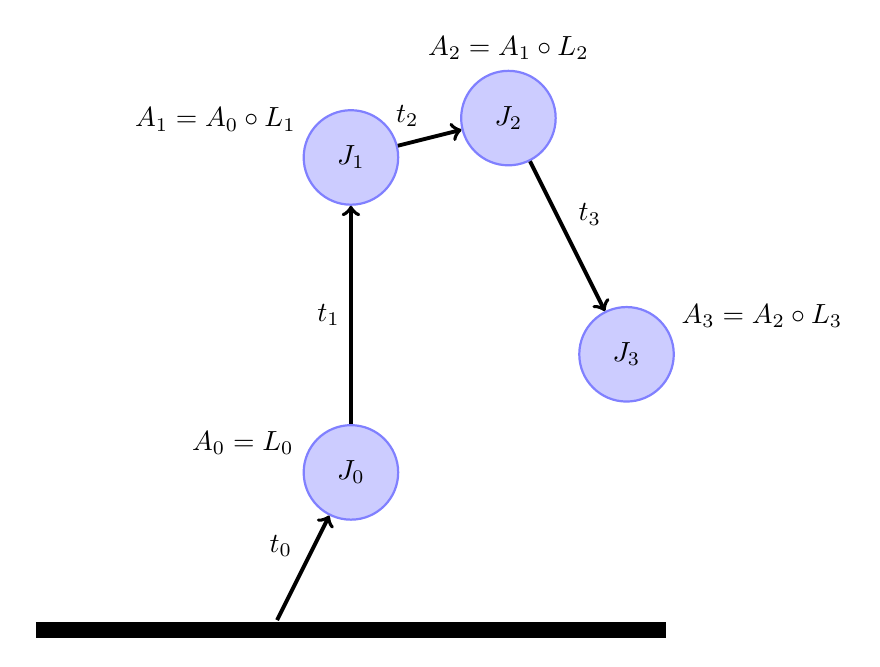
\begin{tikzpicture}
  [joint/.style={shape=ellipse,draw=blue!50,fill=blue!20, thick,
         inner sep=0pt, minimum width=12mm, minimum height=12mm},
  auto
  ]
   \begin{scope}[line width=6pt]

  \draw (-4,0) -- (4,0);
   \end{scope}
  \node (origin) [minimum size = 0] at(-1, 0) {  };
 \path
   (0, 2) node (j0)        [joint, label=170:{$A_0=L_0$}] {$J_0$}
  ++(0, 4)   node (j1)   [joint, label=160:{$A_1=A_0\circ L_1$}]         {$J_1$}
  ++(2, 0.5)   node (j2)    [joint, label=90:{$A_2=A_1\circ L_2$}]         {$J_2$}
  ++(1.5, -3)   node (j3)     [joint, label=20:{$A_3=A_2\circ L_3$}]         {$J_3$}

   ;
   \begin{scope}[line width=1.4pt]
   \draw [->] (origin) to node{$t_0$} (j0);
   \draw [->] (j0) to node{$t_1$}(j1);
   \draw [->] (j1) to node{$t_2$}(j2);
   \draw [->] (j2) to node{$t_3$}(j3);
   \end{scope}

\end{tikzpicture}
\caption{Part of a skeleton, with Translations $t_i$, Local Transforms $D_i$, and global transforms $A_i$}\label{figure:skeletonfragment}
\end{figure} 

\subsubsection{Adjusting bind matrices}

We have seen the generic weight blending equation \ref{eq:weightblending} above.
There are various situations where we would like to modify the (inverse) bind matrices $B_i^{-1}$,
thereby redefining the ``neutral pose'' for a character.
One reason could be that the neutral pose as defined by some 3D modeling tool is inconvenient.
For instance, the neutral position for a Collada export from 3DSMax defines a rather strange looking ``neutral'' position.
Moreover, in such modeling tools the character mesh is often aligned with the Z-axis, (called the ``up-axis'') and for our animation engine
we prefer a world where the Y-axis is the ``up-axis''. A final reason would be
that we want to switch to a \emph{new} neutral position like the one defined by the HAnim standard.
In all such cases, three things have to happen:
\begin{enumerate}
\item The \emph{(inverse) bind matrices} must be changed. This can be done by multiplying $B_i^{-1}$
by matrices $V_i$ that must be chosen in a suitable way for each of the situations mentioned above.
\item The local \emph{rotations} for every joint to be used for various poses in animations must be adapted accordingly.
This step is necessary only when existing animation data that was created for the ``old'' bind matrices.
When new animation data has to be produced it might be much more convenient to work immediately with
the ``new'' bind matrices. For instance, if we switch bind matrices that are suitable for HAnim then
new animation data should use the HAnim pose as ``neutral'' pose. On the other hand, existing animation data,
for instance, data exported from the 3D modeling tool, will be based upon the ``original'' bind matrices, and so
we have to convert the rotations from that data.
\item The local \emph{translations} for every joint must be adapted to the new bind matrix.
This can be done once, since translations and (modified) bind matrices are not changed by animation data.
The only exception here that we allow is the ``humanoid root translation'' $t_0$, for the root joint $J_0$:
this translation is sometimes modified in animations.
\end{enumerate}
%
We discuss here first the generic case, where we multiply $B_i^{-1}$ by arbitrary $V_i$.
We assume here that $V_i$ is just a rotation, and contains no translation.
That means that we replace an inverse bind matrix $B_i^{-1} = U_i^{-1}\,T_{-C_i}$
by ${B'}_i^{-1} = V_i\,U_i^{-1}\,T_{-C_i}$.
We consider some (arbitrary) pose based upon the original bind matrices,
specified by a series of rotations $R_0, R_1, \ldots, R_n$.
For this pose, joint $J_i$ has a global transformation $M_i$ of the form:
%
\[ M_i = T_{t_0}\, R_0\, T_{t_1}\, R_1 \cdots T_{t_i}\, R_i\, U_i^{-1}\, T_{-C_i}\]
%
When we multiply the $U_i^{-1}$ matrices with $V_i$, we must switch to a new set of translation
vectors $t_i'$ and new rotation/scaling matrices $R_i'$, as follows:
%
\[ M_i' = T_{t_0'}\, R_0'\, T_{t_1'}\, R_1' \cdots T_{t_i'}\, R_i'\,  V_i U_i^{-1}\, T_{-C_i}\]
%
We require that $M_i' = M_i$ for all $i$, something we
can realize by making the following choice for $t_i'$ and $R_i'$:
%
\begin{gather}
t_i'= V_{i-1}(t_i)\notag\\
 R_i' = V_{i-1}\,R_i\,V_i^{-1}\notag
\end{gather}
Here, we use the convention that $V_{-1} = Id$.
Imagine some virtual joint $J_{-1}$ with identity transformations,
as parent for the humanoid root node $J_0$.
Note that because of this, the humanoid root translation $t_0$ need \emph{not} to be transformed,
which is in particular convenient when this translation is modified in an animation.
%
\begin{gather}
 M_i' = T_{t_0'}\, R_0'\, T_{t_1'}\, R_1' \cdots T_{t_i'}\, R_i'\, V_i U_i^{-1}T_{-C_i}\notag\\
 = T_{t_0}\,R_0\,V_0^{-1}\,T_{V_0(t_1)}\,V_0\,R_1\,V_1^{-1} \cdots \notag \\
 %   V_{i-1}^{-1}\,T_{V_{i-1}(t_i)}\,V_{i-1}\,R_i\,V_{i}^{-1}\, V_i U_i^{-1}T_{-C_i}\notag\\
 = T_{t_0}\,R_0\,T_{V_0^{-1}(V_0(t_1))}\,V_0^{-1}\,\,V_0\,R_1 \,V_1^{-1}\cdots  \notag \\
  % T_{V_{i-1}^{-1}(V_{i-1}(t_i))}\, V_{i-1}^{-1}\, V_{i-1}\,R_i\,V_{i}^{-1}\, V_i U_i^{-1}T_{-C_i}\notag\\
  = T_{t_0}\,R_0\,T_{t_1}\,R_1 \,V_1^{-1} \,T_{V_1(t_2)} \, V_1\,R_2\,V_2^{-1}\cdots \notag = \cdots\notag \\
  %T_{V_{i-1}^{-1}(V_{i-1}(t_i))}\, V_{i-1}^{-1}\, V_{i-1}\,R_i\,V_{i}^{-1}\, V_i U_i^{-1}T_{-C_i}\notag\\
  = T_{t_0}\,R_0\,T_{t_1}\,R_1\,T_{t_2}\, R_2 \cdots T_{t_i}\,R_i\,V_i^{-1}\,V_i U_{i}^{-1}T_{-C_i}  =\notag\\
   = T_{t_0}\,R_0\,T_{t_1}\,R_1\,T_{t_2}\, R_2 \cdots T_{t_i}\,R_i\,U_{i}^{-1}T_{-C_i}  = M_i\notag
\end{gather}
(This was to be shown.)


\subsubsection{Simplifying bind poses}

The first application of bind pose modification is to \emph{simplify} the bind matrices.
The main reason for this step would be to get rid of overly complicated bind matrices introduced
by tools like the Collada exported for 3DSMax: the original ``neutral'' pose looks incomprehensible.
Before we start simplifying we have a more detailed look at bind poses and bind matrices.
Let's assume that, in order to put the skeleton in the bind pose, we must apply
\emph{local} joint transformations of the form $T_{t_i} L_i$, where $t_i$ is a local translation, and $L_i$ is a local
rotation (and possibly scaling).
We consider the concatenation of such transformations along a path within the skeleton, starting at
the humanoid root, and ending in some joint $J_i$.
For convenience we assume here that this chain consists of joints $J_0, J_1, J_2, \ldots, J_i$.
The  global transform for  joint $i$ for the bind pose  must be equal to $B_i$.
For in that case, it will be canceled by the inverse bind matrix $B_i^{-1}$, and effectively we have \emph{no}
transformation of the mesh. And the pose where there is no transformation is (by definition) the bind pose.
 Therefore, we see that
 %
 \[ T_{t_0} L_0 T_{t_1} L_1 \cdots T_{t_i} L_i = B_i = T_{C_i} U_i.\]
%
The left hand side of this equation can be rewritten as $T_t L$, where:
\begin{gather}
 L = L_0 L_1\cdots L_i = U_i. \notag \\
 t = t_0 + L_0(t_1) + \cdots + L_0 L_1\cdots L_{i-1}(t_i) \notag\\
  = t_0 + U_0(t_1) + \cdots + U_{i-1}(t_i) = C_i \notag
\end{gather}
%
The easiest way to simplify bind matrices is
to replace bind matricies of the form $B_i = T_{C_i} U_i$ by  new
bind matrices ${B'}_i = T_{C_i}$. So, basically, we want to drop the rotation and scaling parts $U_i$ altogether,
so that only a translations remains.
Clearly, what must be done is to multiply $B_i^{-1}$ by $U_i$, for in that case we have that
${B'}_i^{-1} = U_i U_i^{-1} T_{-C_i} = T_{-C_i}$, which is the desired inverse bind matrix.
From the previous section we now see that we must adapt local translations $t_i$ and rotation $R_i$
as follows:
\begin{gather}
t_i'= U_{i-1}(t_i)\notag\\
R_i' = U_{i-1}\,R_i\,U_i^{-1}\notag
\end{gather}
%
From the equation above for $t = \cdots = C_i$, we see that $t_i' = C_i - C_{i-1}$
So the modified translation vector $t_i'$ is simply the translation vector from the center position
of joint $J_{i-1}$ to the center position of joint $J_i$ within the bind pose.

\subsubsection{Reorienting your avatar}
The next step that we want to discuss is how to re-orient mesh data. What we want is an avatar
with its mesh and skeleton aligned with the Y-axis, looking into the positive Z-axis direction.
Slightly more general, we want to apply some (linear) coordinate transform $R$ to the mesh, skeleton,
and animation poses. For example, if we have some avatar with mesh and skeleton aligned with the Z-axis,
and some pose where the shoulder joint rotates $-45^\circ$ around the Y-axis,
then after the coordinate transform we have a mesh and skeleton aligned with the Y-axis, and the same
pose now has a shoulder joint rotation of $+45^\circ$ around the Z-axis.
In this case, the coordinate transform $a$ is a rotation of $-90^\circ$ around the X-axis.

Assume that we have some linear coordinate transform $R$. Usually, $R$ will be a rotation, but it
could include scaling.
We want to transform mesh coordinates $v$ into $v' =R(v)$, and then later on use our adapted skeleton
to operate on this transformed mesh.
The question now is: how to adapt the skeleton and animation poses.

Assume that some pose is described by local affine joint transforms $D_i$ which
describe local joint pose like the shoulder joint in the example above.
Within the new coordinates, the effect of $D_i$ will be achieved
by $D'_i = R\:D_i\:R^{-1}$.
(Just examine the effect of $D'_i$ on some ``new'' coordinate of the form $v' = R(v)$. The result is that
$D'_i(v') = R\:D_i\:R^{-1} (R(v)) = R\:D_i(v)$.)
Of course this is to be expected: $R\:D_i\:R^{-1}$ is just the standard linear algebra result
for how matrices change under coordinate transforms.
Now we must take into account that the local transforms $D_i$ that describe some pose
are affine transforms of the form $D_i = T_{t_i}\:L_i$ where $t_i$ is the (fixed) local skeleton translation
from the parent of joint $J_i$ to $J_i$ itself, and where $L_i$ is the (changing) rotation matrix for joint $J_i$.
We can rewrite the  $D'_i$:
\begin{equation}
D'_i = R\:D_i\:R^{-1} = R\:T_{t_i}\,L_i\:R^{-1}
=R\,T_{t_i}\,R^{-1}\:R\,L_i\,R^{-1}.
\end{equation}
The rightmost three factors, i.e. $R,L_i\,R^{-1}$, are just the transformed rotations $L'_i$, adapted to
the new coordinate system. For instance, if $L_i$ would be the $-45^\circ$ around the Y-axis from the example
above, and $R$ would be the coordinate transform defined by a $-90^\circ$ rotation around the X-axis,
then $R\:L_i\:R^{-1}$ is actually the $+45^\circ$ around the Z-axis, as expected.

\noindent
The left most factors, i.e. $R\,T_{t_i}\,R^{-1}$ are the modified translations.
We can simplify this considerably:
\begin{equation}\label{eq:transormedtranslation}
R\:T_{t_i}\:R^{-1}
=T_{R(t_i)}\:R\:R^{-1}
=T_{R(t_i)}
\end{equation}

\noindent
Finally, we can see how this all fits together, when we apply an linear transform $R$ to
a mesh that is being deformed by means of weight blending, specified by \autoref{eq:weightblending}.
We assume that  $A_i = T_{t_i}\,L_i$, that $B_i^{-1} = U_i\,T_{-C_i}$.
We denote by $L'_i$ the transformed $L_i$, that is, $R\,L_i\,R^{-1}$.
 Similarly  we define ${U'}_i^{-1} = R\,U_i^{-1}\,R^{-1}$.
Then the result of applying $R$ yields the following transformed blend equation:
%
\begin{equation}
 R \:\sum_{i=0}^{n} w_i\, A_i\,B_i^{-1} = \sum_{i=0}^{n} w_i\, R\,A_i\,B_i^{-1} \quad\text{, where}\notag
 \end{equation}
 %
 \begin{gather}
 R\,A_i\,B_i^{-1} = \notag\\
 R\,T_{t_0}\,L_0\,T_{t_1}\,L_1\cdots T_{t_i}\,L_i,U_i^{-1}\,T_{-C_i}=\notag\\
 R\,T_{t_0}\,R^{-1}\,R\,L_0\,R^{-1}\,R\,T_{t_1}\,L_1\cdots T_{t_i}\,L_i\,U_i^{-1}\,T_{-C_i} =\notag\\
 T_{R(t_0)}\,L'_0\, R T_{t_1}\,L_1\cdots T_{t_i}\,L_i\,U_i\,T_{-C_i} =\cdots=\notag\\
 T_{R(t_0)}\,L'_0\,T_{R(t_1)}\,L'_1\cdots T_{R(t_i)}\,L'_i\,U'_i\,T_{R(-C_i)}\,R\notag
 \end{gather}
 %
 The remaining $R$ at the right end of this last formula is the transform to be applied on the mesh.

 We conclude that, apart from transforming the mesh by means of applying $R$ to the vertices,
 we need to adapt translation vectors $t_i$, rotation/scaling matrices $L_i$,
 and the  as follows:
\begin{gather}
t_i'= R(t_i)\notag\\
L_i' = R\,L_i\,R^{-1}\notag\\
C_i' = R(C_i)\notag\\
U_i' = R^{-1} U_i R
\end{gather}

 Since the translations, and the bind matrices are fixed, they can be calculated before we start rendering.
 This is very similar to the transformations for simplifying the bind matrix.
 What is different is that the translation part of the bind matrix is also modified



\subsubsection{Redefining the avatar neutral pose}

The result of the previous sections is an avatar where the original bind pose is also the neutral pose,
that is, when all local rotation matrices are set to identity, the avatar will assume a pose equal to
the bind pose. We would like to change this, and define some other pose, say the HAnim pose,
to be the neutral pose.
This problem can be split into two steps:
\begin{enumerate}
\item First, find out how to put the avatar in the HAnim pose,
\item Second, define that pose as the neutral pose, by adapting transformations and bind matrices.
\end{enumerate}
%
We start with the second step, so, we assume that we have a a pose defined by local rotations (and possibly scaling) $H_i$
that define a pose that we would like to set as the neutral pose.
Using the existing bind matrices and translation vectors, the global transform for joint $J_i$ for this new neutral pose is:
%
\begin{equation}
T(t_0)\,H_0\,T(t_1)\,H_1\,T(t_2)\, L_2\cdots T(t_i)\,H_i\,B_i^{-1}\notag
\end{equation}
%

We would like to modify the bind matrices in such a way that we can represent the same pose using \emph{identity}
matrices replacing the $H_i$ matrices.
This can be achieved by using new inverse bind matrices ${B'_i}^{-1}$ and new translation vectors $t_i'$ of the form
\begin{gather}
{B'_i}^{-1} = V_i B_i^{-1} \notag\\
t_i' = V_{i-1}(t_i) \textrm{, where} \notag \\
V_i = H_0 H_1 \cdots H_i\notag\\
\end{gather}
%
Also, an existing (arbitrary) animation pose, defined by rotations/scalings \\
$R_0, R_1, \ldots , R_n$, must be replaced by an adapted pose $R_0', R_1', \ldots, R_n'$ where:
 \[R_i' = V_{i-1} R_i V_i^{-1} \notag.\]


For the \emph{first} step, i.e. putting some skeleton in the HAnim pose, one can use various techniques;
in the end, all that count is that our VH is in the desired pose.
For a pose like the HAnim standard, it is often useful to have a method that aligns specified segments
of the human body with direction vectors $\mathit{dir}$. For example, the HAnim standard requires that upper and lower arm
are ``hanging downwards'', i.e. are aligned with the direction of the (negative) Y-axis.
In this case, we would align those segments with a direction vector $(0, -1, 0)$.
Let us assume that we have determined that the current situation of the body is such that we
have two joints, a parent and a child, and that the segment in between those two joints is currently
aligned with some vector $a$.
It is easy to establish a quaternion that rotates $a$ into $\mathit{dir}$.
(We assume that both $a$ and $\mathit{dir}$ are normalized vectors, i.e. $|a| = |\mathit{dir}| = 1$:
Let $h = ( (a+\mathit{dir})/ |a+\mathit{dir}|)$. (That is, $h$ is the normalized half-vector in between $a$ and $\mathit{dir}$.)
Now q is simply $(a\cdot h, a\times h)$. We are not done yet, since we now know how to rotate our segment \emph{after} that segment
has been rotated by the skeleton transforms. Let us denote the latter rotation by a quaternion $r$.
Then our construction delivers a quaternion $q$ as above, with the property that $q\,r$ is a rotation that puts our segment
in the desired orientation. Here, $r$ itself is a product like $r = r_0 r_1, \cdots r_n$, where the quaternions $r_i$ are
the current (local) rotations of the skeleton joints, starting at the root, up to and including the parent joint rotation.
 What we want instead is a quaternion $s$ with the property $q\, r = r\, s$,
for in that case, we can replace the local quaternion $r_n$ by $r_n\, s$, i.e. a post multiplication
of the local parent joint rotation $r_n$  with the $s$ quaternion. From the equation it follows
that $ s= r^{-1}\, q\,r$. (Basically, this is is $q$ rotated by $r^{-1}$.)










%\input{\hmigraphicsreportdir/hmi-graphics-scenegraph.tex}
%\input{\hmigraphicsreportdir/hmi-graphics-collada.tex}
%
\section{OpenGL}

The hmi.graphics.opengl package defines a basic render engine based upon the Jogl binding for OpenGL.

\begin{itemize}
\item GLRenderContext: wrapper class for a Jogl GL object. This is the Jogl defined interface to OpenGL functionality.
In addition a GLRenderContext can define extra render state information, such as
the current \emph{renderpass}.
\item GLRenderObject: Interface for all objects that can be ``rendered'' using an OpenGL render context.
The two methods: glInit and glRender are called with a GLRenderContext parameter that includes
a Jogl GL object with what is called a \emph{current} OpenGL context.

\item GLRenderList: Basically a List of GLRenderObjects, that can be treated as a GLRenderObject itself.

\item GLShape: An GLRenderObject that defines, by means of a user specified GLRenderList,  an OpenGL render state,
that defines geometry by means of a second user defined GLRenderList, and
that defines a transform matrix to be applied to the geometry.
The render state objects are ``rendered'' only nor non-shadow passes, and they are rendered
immediately before the geometry.
The render state settings are ``additive'', that is, they will affect the current OpenGL state,
but there is no pop/push mechanism for restoring the old state after rendering.
The transformation on the other hand is passed on to OpenGL by means of the OpenGL glPushMatrix/glPopMatrix
mechanism. The matrix itself should be in row-major order. (It is multiplied with the OpenGL modelview matrix
by means of glMultTransposeMatrix, to conform to OpenGL's column-major matrix order.)
The transform matrix is \emph{not} kept inside the GLShape object. Rather, it is a reference to a matrix
elsewhere, typically inside a VJoint object from hmi.animation.

\item GLBasicMesh: A GLRenderObject that defines a simple geometry ``mesh''.
It defines a number of OpenGL vertex attributes and a (shared) index structure.
The attributes are kept in objects of type GLVertexAttribute.
The vertices should be arranged by means of triangles.

\item SkinnedMesh: an extension of GLBasicMesh that can handle meshes which can be
\emph{modified} or \emph{deformed} real-time by means of a skeleton based technique.
It keeps references to several transform matrices (one for every skeleton joint), and
uses some extra vertex attributes like joint indices and joint weights.
Since it must deform the \emph{original} vertex data, it keeps copies of these original
data arrays for vertex coordinates and vertex normals.

\item GLVertexAttribute: helper class for GLBasicMesh. Basically a wrapper for
a java.nio.FloatBuffer containing the raw data for one OpenGL vertex attribute.
This data can be initialized in various ways, for instance, by copying from a hmi.scenegraph.VertexAttribute object.
GLVertexAttribute deals with the complex OpenGL attributes ``old style'', as well as with attributes
for more modern shader programming.

\item GLUtil: a basic util, for reporting GL errors etcetera.

\item Renderer4: A basic top-level ``render engine'' that deals with the obligatory Jogl setup.
So it defines the Jogl GLEventListener interface, deals with Jogl generated events
like int(), display(), displayChanged(), and reshape(). It will \emph{cause} a Jogl display call
whenever it receives a time() call, typically  from a hmi.util.SystemClock. Then, upon receiving
the (self-indiced) Jogl display call, it will start a render phase by calling the glRender() method
for a top-level GLRenderObject, that is called the ``scene''.
A few display settings can be made: the near and far plane, and the field-of-view angle.

\end{itemize}

\subsection{Package: hmi.graphics.opengl.scenegraph}

Although the opengl package can be used for ``standalone'' OpenGL demo programs,
it will typically be part of a larger setup, where the graphics is being defined using
the hmi.graphics.scenegraph package. OpenGL is not a scene graph api, therefore the scenegraph related
elements of the render engine have been placed in a special package: hmi.graphics.opengl.scenegraph.
This package mainly includes classes for the \emph{compilation} from hmi.grapgics.scenegraph structures
to hmi.graphics.opengl structures. But it also contains a few scenegraph classes: VGLNode
and VGLRenderStruct. These classes are based not only on the opengl classes, but also on hmi.animation.VJoint.

\begin{itemize}
\item VGLNode: A GLRenderObject containing a VJoint that defines a transform matrix, and a GLRenderList
containing GLRenderObjects, to be rendered with a OpenGL modelview matrix defined by the VJoint.
A VGLNode is a scenegraph node: you can \emph{add}  child VGLNodes. The effect
of an addChild operation is to create a VJoint parent-child relationship, and to
simply \emph{combine} the GLRenderLists. Of course, one would typically expect the GLRenderObjects
to refer to matrices from the VJoint tree.

\item GLScene: ``work under construction''. The idea is that VGLNodes are not quite sufficient
when complete Collada-like structures have to be dealt with.
So, we have a GLScene that should keep the ``top-level'' structures:
a list of ``root'' VJoints, a list of GLShapes, a list of SkinnedMeshes.



\end{itemize}



%
\section{Compilation}

Compilation (currently) is relevant for the following stages:
\begin{enumerate}
\item From the hmi.graphics.collada format to hmi.graphics.scenegraph format.
This step is carried out by classes inside the hmi.graphics.collada.scenegraph package.
The idea is that after the compilation, we end up with a ``neutral'', graphics format independant description of a graphics scene.
This stage is independant from the opengl related classes.
\item From the hmi.graphics.scenegraph format to hmi.graphics.opengl format.
This stage is carried out by the hmi.graphics.opengl.scenegraph package. Since it compiles
from scenegraph format, it is independent from graphics file formats.
\end{enumerate}

The first step deals with compiling a subset of the very general Collada format into
the more regular scenegraph format. The second step compiles into a low-level OpenGL format.
As can be seen, the two steps follow logically one after another, yet, the intermediate scenegraph format
is \emph{not} dependent on either the Collada format or the OpenGL related packages.
The (future) idea is to extend the approach, in particular to allow more graphic formats,
all to be compiled into the scenegraph format. In principle, the second step could also be replaced by compiling
into something else, like Java3D, OpenGL ES etcetera.

In this section we discuss both compilation steps \emph{together}, without all of the details,
in order to see how a Collada scene ends up eventually as data structures for the Jogl renderer.
















\subsection{hmi.graphics.opengl ``controllers'' and hmi.animation ``skeletons''}

The counterpart of Collada's skin controllers at the OpenGL/Jogl level is the combination
of GLSkinnedMesh objects combined with skeleton structures in the form of trees of VJoint objects.
It is important here that skeletons and VJoints are part of the hmi.animation package, \emph{not} part of any of
the hmi.graphics packages. The rationale here was to keep ``animation'' as such independent from OpenGL implementation
issues. (The hmi.animation package can even be compiled without hmi.graphics available)

The most important points:
\begin{itemize}
\item A \verb"GLBasicmesh" defines vertex attributes like vertex coordinates, texture coordinates, normals, colors,
or more general GLSL shader attributes. It does \emph{not} deal with bone structures, skeletons, skin weights etcetera.
\item A \verb"GLSkinnedMesh" is an extension of a \verb"GLBasicMesh", and adds skinning information.
\item More in particular, a \verb"GLSkinnedMesh" defines: joint indices and joint weights per vertex, vcounts,
for the number of joint/weights per vertex, joint matrices, inverse bind matrices, joint names and skeleton id.
\item The joint matrices for a \verb"GLSkinnedMesh" are \emph{references} to matrices kept elsewhere.
Typically, each joint matrix will be a reference to a (global) matrix exported by a \verb"VJoint" object.
The rules of the game are that a \verb"GLSkinnedMesh" will read but not modify its joint matrices.
Moreover, it is expected that updates to these matrices will be performed in a way that avoids concurrency problems.
In practice this means that the thread \emph{setting} the values of VJoint matrices must
synchronize by means ofa common lock or common monitor with the thread being used for mesh deformation and rendering.
\item Inverse bind matrices are part of a \verb"GLSkinnedMesh". They are multiplied with the joint matrices
by  calling the \verb"calculateMatrices" method of a \verb"GLSkinnedMesh" object. This should be done
before the \verb"deform" method is being called on such a \verb"GLSkinnedMesh" object.
Note that inverse bind matrices are always needed, even when the bind pose involves only ``trivial'' rotations.
In that case all 3X3 rotation matrices would be identity matrices, but the \emph{translation} from one joint to the next
is still part of the 4X4 (inverse) bind matrix.

\subsection {hmi.graphics.scenegraph ``controllers''}

A (hmi.grapics.)scenegraph defines \verb"GMesh" as the counterpart of Collada's skinned meshes, and opengl's deformable meshes.
A \verb"GMesh" defines normal vertex attributes like vertex coordinates etcetera, but also a special purpose
\verb"VertexWeights" attribute, joint names, s skeleton id, and inverse bind matrices.
The skeleton id is the id of some \verb"GNode" within the scenegraph, that still has to be resolved.
Once this skeleton ``root'' node has been determined, it is assumed that joint \verb"GNode"s can be located
as (recursive) children, by means of their \verb"sid" attribute, that should correspond to the joint names
from the \verb"GMesh".


\subsection{Compiling ``Controllers''}

A Collada \verb"instance_controller"  is compiled into a \verb"GMesh".
All controller information, like joint names, skeleton id, inverse bind matrices, skin mesh, and
skinning information like weights are put into the \verb"Gmesh" object. (We assume here only one skeleton per
\verb"instance_controller")
At the same time, the scene graph's \verb"GNode"s can be compiled into a similar \verb"VJoint" structure.
It has not yet been decided what to do with potential ``sharing'' within scenegraphs, that is, for the moment
we assume tree-like structures, no ``dag'' like scene graphs.
Checking and resolving the skeleton \verb"id" or the joint name \verb"sid"'s can then be done.
In the next compilation step, a \verb"GMesh" can be compiled into a \verb"GLSkinnedMesh"
\end{itemize}


\subsection{Detailed steps for compiling skinned meshes}

A Collada skinned mesh is created by means of an \verb"instance_controller", specifying an url to the geometric mesh
as well as specifying a skeleton node. The mesh geometry itself is a child of the \verb"instance_controller" node,
which is quite independent from the skeleton node. In studio-max exports the skeleton typically resides in a completely separate scenegraph branch, and is the (only) child of some ``Bip'' root node.
Example of an instance controller, referring to the \verb"CWom0023-Pelvis-node" skeleton, and
using a geometric mesh, referenced here as \verb"CWom0023-Mesh".
\begin{verbatim}
<node id="CWom0023-Mesh-node" name="CWom0023-Mesh" type="NODE">
  <instance_controller url="#CWom0023-Mesh-mesh-skin">
    <skeleton>#CWom0023-Pelvis-node</skeleton-->
      ... (instance_material)
  </instance_controller>
</node>
\end{verbatim}

The skeleton, starting at the \verb"CWom0023-Pelvis-node" node, resides in the second secengraph branch,
with root node \verb"CWom0023-Bip-node". 
\begin{verbatim}
  
<node id="CWom0023-Bip-node" name="CWom0023-Bip" type="JOINT">
  <matrix>
     0 1 0 -0.000068 
    -1 0 0  0.016062 
     0 0 1  0.905944 
     0 0 0  1
  </matrix>
  <node id="CWom0023-Pelvis-node" name="CWom0023-Pelvis" sid="Bone1" type="JOINT">
    <matrix>
      0 1 0 -0.007917 
      0 0 1  0 
      1 0 0  0 
      0 0 0  1
   </matrix>
    <node id="CWom0023-Spine-node" name="CWom0023-Spine" sid="Bone2" type="JOINT">
      ... (remainder of skeleton graph)
\end{verbatim}

Note that the skeleton is rotated (and translated as a whole), by means of the pelvis node matrix. 

The mesh itself has (in this example) no inherent transformation, but the Collada idea is that the 
\verb"CWom0023-Mesh-node" could be moved around, affecting the position and orientation of the mesh as a whole. 
So the mesh deformation process, using the skeleton joint nodes, is decoupled from the mesh transformation
as a whole. Still the translation and rotation of the skeleton root or the ``Bip'' node will also
affect this ``global'' position and orientation. 
The skeleton structure specifies a hierarchical tree of joint nodes, each with a local translation, local rotation, and possibly, local scaling. In addition the mesh defines ``inverse bind matrices'', 
and even a \verb"bind_shape_matrix" element. The latter is rather simple: it specifies
a single matrix, to be applied to the mesh geometry in order to get it into 
the so-called ``bind pose''. 
The inverse bind matrices (one per joint) are more complex. 
In essence, they specify the matrices that where needed to get the skeleton structure
into the bind pose as well. For example, consider a skeleton that would have its arms 
hanging downwards, but, on the other hand, a mesh that in the bind pose has the avatar
in the ``T-shape'' pose, with the arms stretched horizontally. 
Then the bind pose for the skeleton would rotate the arms such that they would also be in
a T-shape pose, matching the mesh bind pose. Note that the bind matrix for some joint specifies
the \emph{global} transformation for that joint in order to be in the bind pose, not just
its \emph{local} translation and rotation. 

\subsubsection{ translation steps (``under revision'') }

\begin{enumerate}
\item The Collada package includes classa that mimic the Collada structures quite closely.
The relevant classes here (from \verb"hmi.graphics.collada") are: 
\begin{itemize}
\item \verb"Instance_Controller" : defines the mesh url, and the skeleton ids, via the associated \verb"Skeleton"
\item \verb"Skeleton" : just the url of some skeleton id
\item \verb"Controller" : just a link to the \verb"Skin"
\item \verb"Skin" : the \verb"Joints", \verb"Vertex_Weights", the \verb"Bind_Shape_Matrix"
\item \verb"Joints" : defines the SID's of the joints, as well as the associated inverse bind matrices.
\end{itemize}

\item The hmi.graphics.scenegraph package represents skinned meshes using the following classes:
\begin{itemize}
\item \verb"GNode" : the basic scenegraph node, used used here to represent skeleton joint nodes.
\item \verb"GSkinnedMesh" : keeps track of skeleton ids, joint names, joint sid's, inverse bind matrices,
vertex weights, and links to the skeleton GNode nodes that represent skeleton nodes. 
A \verb"GSkinnedMesh" is an extension of a \verb"GMesh"
\item \verb"GMesh" : represents the mesh geometry, by means of vertex attributes, and vertex index data.
\item \verb"VertexAttribute" : a generic vertex attribute, like position, normal, texture coordinate, color
\item \verb"VertexWeights" : somewhat like a complicated \verb"VertexAttribute", keeping track
of vertex weights for a \verb"GSkinnedMesh". 
\end{itemize}




\item The scenegraph structures are not directly fit for rendering in an OpenGL context.
The \verb"hmi.graphics.opengl" package contains OpenGL based counterparts for scenegraph structures.
The relevant classes for skinned meshes are:
\begin{itemize}
\item \verb"GLSkinnedMesh" : defines OpenGL vertex attributes and index data, joint matrices,
inverse bind matrices. (For debugging purposes it also keeps track of joint names etc.)
\verb"GLSkinnedMesh" is an extension of \verb"GLBasicmesh" 
It knows how to \emph{deform} the mesh data from the underlying \verb"GLBasicMesh", based upon the
current joint matrices, inverse bind matrices, and vertex weights.
\item \verb"GLBasicMesh" : keeps track of vertex attributes and vertex index data.
In particular it knows how to render the mesh, using this data.
\item \verb"GLVertexAttribute" : auxiliary class, used by \verb"GLBasicMesh" to deal
with vertex attribute data.
\end{itemize}


\item The translation from Collada structures to scenegraph structures:\\
The translation methods are located within the \verb"hmi.graphics.collada.scenegraph" subpackage.
The translation here boils down down to collecting information that is spread around within the Collada
structures, and combining it into  \verb"GSkinnedMesh" objects, together
with \verb"GNode" based skeleton graphs. The transformation part of a Collada node is transformed into
a \verb"VJoint" that is kept inside a scenegraph  \verb"GNode". 
Since both \verb"VJoint" structures and \verb"GNode" structures
are hierarchical trees, we have some (unfortunate) hierarchy duplication here. 
A slight advantage is that the \verb"VJoint" based structure is based solely upon
the \verb"hmi.animation" package, and is quite independant from the \verb"hmi.graphics" packages.

Note that a single Collada mesh can consist of more than one ``primitive'', where a primitive in this context 
is a part of the mesh geometry together with a material. Such primitives are currently translate
into separate \verb"GSkinnedMesh" objects, that typically share a single skeleton structure.


The translation at the highest level compiles a complete Collada document into a \verb"GScene" object.
The latter collects global information like the root nodes of the scenegraph, but also keeps track of 
all \verb"GSkinnedMesh" es that occur within the scene.
In a second translation step these \verb"GSkinnedMesh"es are worked on in order to
get them prepare them for rendering in the OpenGL framwork, and in order to simplify animation.
For instance, exported skinned meshes are often in the wrong orientation (lying on the ground),
are not based upon the default HAnim skeleton structure and poses, might include scaling operations
which complicate matters etcetera. The \verb"GScene" methods are meant to deal with all this. 

Here is what we would like:
\begin{enumerate}
\item The avatar is standing at the origin, upright, where ``up'' means in the positive Y-direction
\item All joints have been resolved in the sense that they are coupled to the appropriate \verb"GNode".
\item the joint names are the standardized HAnim joint names, and the joint structure conforms to the
HAnim standard. 
\item The default pose, that is, the pose where all local joint rotations have been set to 
the identity matrix, is the default HAnim pose, where for instance arms are pointing downwards,
and are aligned with the Y-axis. 
\item There is no scaling. In particular, we don't like non-uniform scaling, but other forms of scaling are also
not convenient.

\end{enumerate}

In order to achieve this, the following steps are taken:

\begin{enumerate}
\item joints are resolved: skeleton ids are used to find corresponding skeleton root nodes inside
the scenegraph \verb"GNode" branches, then joint \verb"GNode"s are searched for by sid 
within the sub tree(s) defined by these root node(s).
When found the GSkinned mesh is linked to the global matrix of the VJoint of the skeleton GNode.
This direct coupling means that during rendering the GNode structure is no longer needed: the 
mesh will use the global matrix of the joint directly. 
For convenience, we copy the joint names from the skeleton nodes to the GSkinned mesh, mainly for debugging purposes.
\item In the second step, joint sids (and joint names) are \emph{renamed}, based upon a user specified
renaming list. The renaming is carried out both on the GSkinnedMeshes as well as the GNodes from the skeletons.
This ``early renaming' guarantees that later stages can assume, for instance, that HAnim joint sids/names
are being used. The original joint ids are \emph{not} renamed. 

\item the next step is to rotate and scale the mesh as a whole. Say, your mesh is specified with centimeters,
rather than with meters. Then you want to scale by a factor $1/100$. If the avatar
is lying on its nose, in the direction of the Z-axis, you want to rotate it such that the Y-axis is the ``up-axis''.
This step actually modifies the geometric attributes of the mesh
\end{enumerate}

\item The translation from scenegraph structures to opengl structures:\\

Here we translate  \verb"GSkinnedMesh" objects into  \verb"GLSkinnedMesh" objects,
\verb"GNode" objects into a \verb"GShape" objects.
The \verb"VJoint" object that represents
the transformation aspect of a \verb"GNode" are kept, and form the transformation scenegraph during rendering.



\end{enumerate}





\end{document}

